\section{Bộ vi xử lý trên từng nền tảng}

\paragraph{}{Mặc dù có cấu trúc chung, bộ vi xử lý được tối ưu hóa khác nhau cho từng loại hệ thống:}

\subsection{Bộ vi xử lý máy tính cá nhân (PC CPU)}

\begin{itemize}
    \item \textbf{Đặc điểm chính}: Cân bằng giữa hiệu năng, giá thành và khả năng xử lý đa dạng các tác vụ từ văn phòng, duyệt web, giải trí đa phương tiện đến chơi game và các ứng dụng đồ họa chuyên sâu.
    \item \textbf{Kiến trúc phổ biến}: Chủ yếu là kiến trúc x86 (và x86-64) do Intel và AMD phát triển. Đây là kiến trúc tập lệnh phức tạp (CISC - Complex Instruction Set Computer).
    
    \item \textbf{Số lõi/luồng}: Thường có từ 2 đến 16 lõi (cores), với công nghệ siêu phân luồng (Hyper-Threading của Intel hoặc SMT của AMD) cho phép mỗi lõi vật lý xử lý nhiều luồng (threads) đồng thời, tăng hiệu suất đa nhiệm.
    
    \item \textbf{Cache}: Có đủ các cấp cache (L1, L2, L3) với dung lượng đáng kể để đáp ứng nhu cầu xử lý đa dạng.
    
    \item \textbf{Tích hợp Đồ họa (Integrated Graphics - iGPU)}: Nhiều CPU PC hiện đại tích hợp sẵn nhân xử lý đồ họa, đủ cho các tác vụ cơ bản và một số game nhẹ, giảm chi phí cho card đồ họa rời.
    
    \item \textbf{Khả năng ép xung (Overclocking)}: Một số dòng CPU cho phép người dùng tăng tốc độ xung nhịp để đạt hiệu năng cao hơn, đòi hỏi hệ thống tản nhiệt tốt.
    
    \item \textbf{Quản lý năng lượng}: Các tính năng quản lý năng lượng ngày càng được chú trọng để tối ưu hóa hiệu suất trên từng Watt điện tiêu thụ, đặc biệt quan trọng cho laptop.
\end{itemize}

\begin{figure}[H]
    \centering
    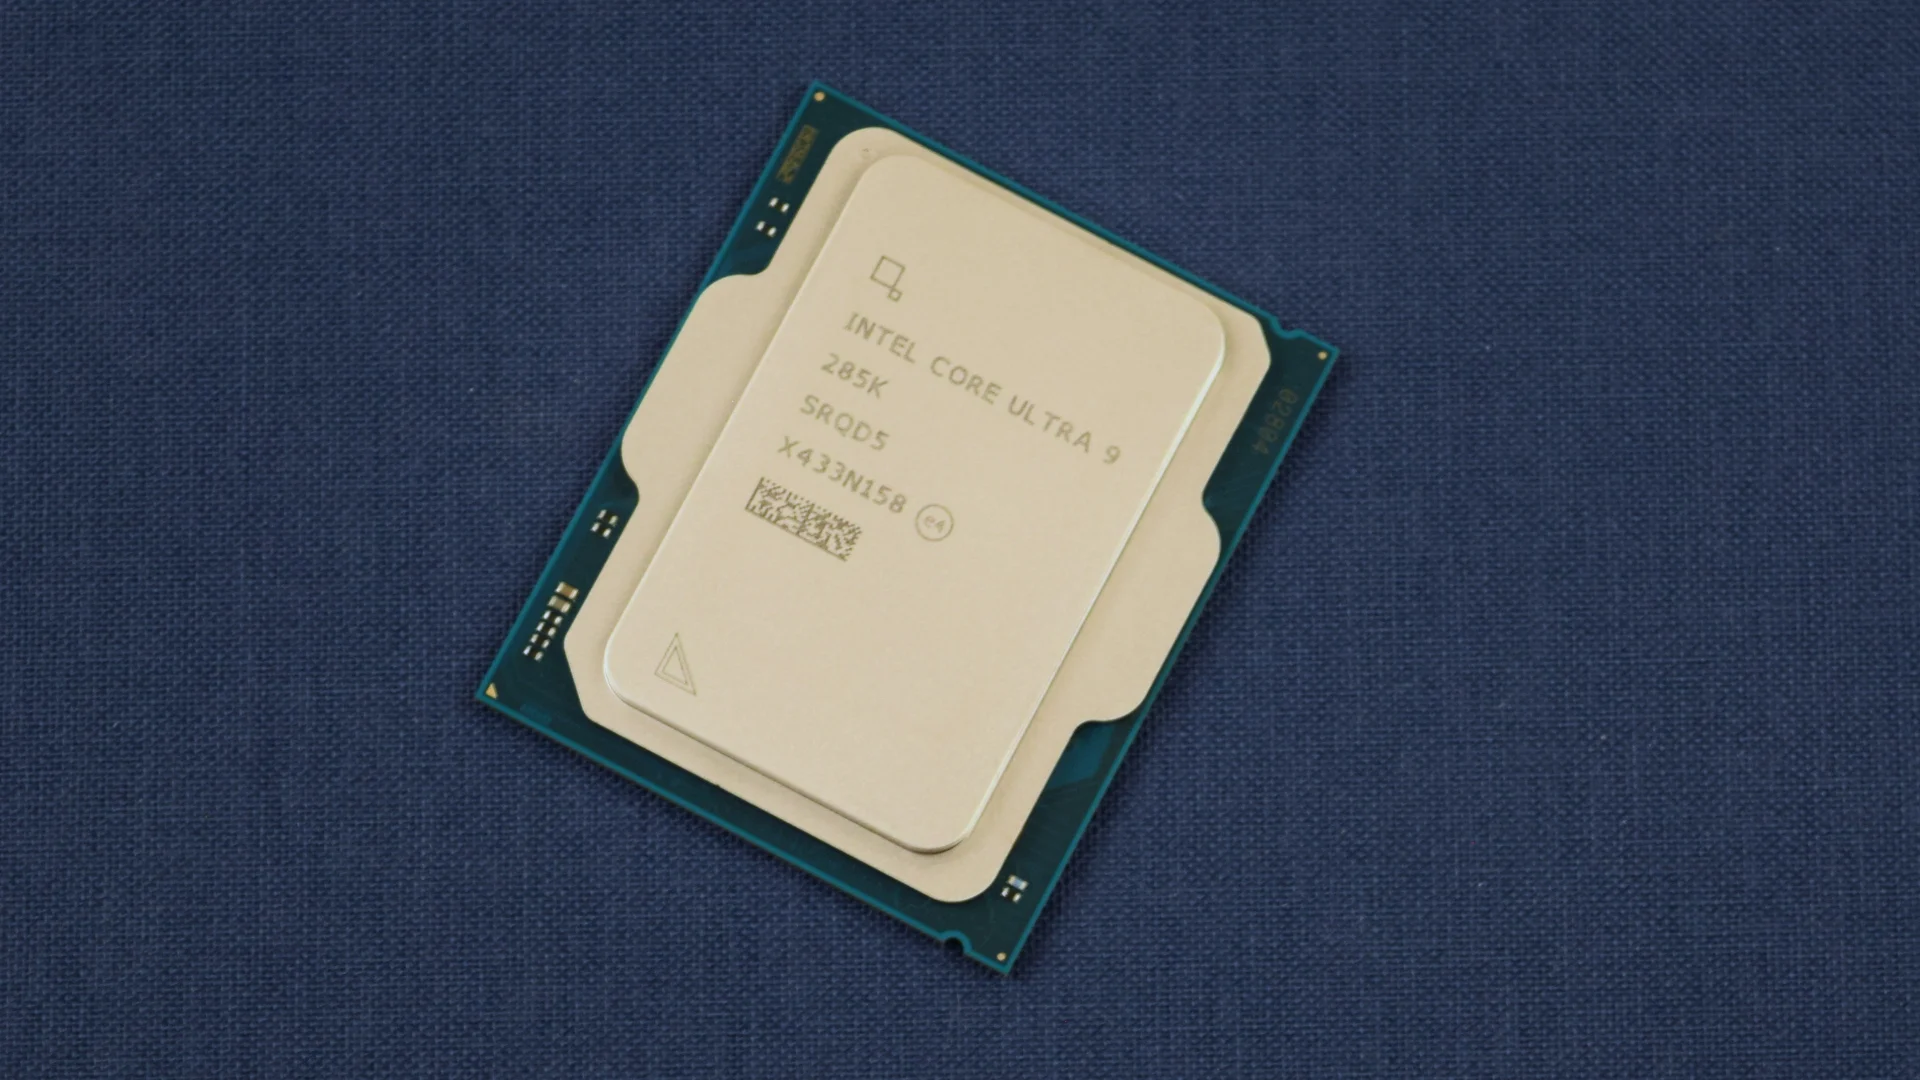
\includegraphics[width=0.85\linewidth]{img/cpu_pc.png}
    \caption{Bộ xử lý Intel® Core™ Ultra 9 285K - một trong những CPU PC mạnh nhất hiện nay}
\end{figure}

\subsection{Bộ vi xử lý máy chủ (Server CPU)}

\begin{itemize}
    \item \textbf{Đặc điểm chính}: Ưu tiên độ tin cậy, tính sẵn sàng cao (hoạt động liên tục 24/7), khả năng xử lý song song mạnh mẽ, băng thông bộ nhớ lớn và các tính năng hỗ trợ ảo hóa, bảo mật cấp doanh nghiệp.
    
    \item \textbf{Kiến trúc phổ biến}: Kiến trúc x86-64 vẫn chiếm ưu thế (ví dụ: Intel Xeon, AMD EPYC). Kiến trúc ARM cũng đang dần xuất hiện trong một số phân khúc máy chủ nhờ ưu thế về tiết kiệm năng lượng.

    \item \textbf{Số lõi/luồng}: Số lượng lõi và luồng rất lớn, có thể lên đến hàng chục hoặc hàng trăm lõi trên một CPU, hoặc hệ thống đa CPU (multi-socket) để xử lý đồng thời lượng lớn yêu cầu từ nhiều người dùng hoặc ứng dụng.

    \item \textbf{Cache}: Dung lượng cache, đặc biệt là L3 cache, rất lớn để phục vụ khối lượng công việc nặng và giảm độ trễ truy cập dữ liệu.

    \item \textbf{Hỗ trợ RAM ECC (Error-Correcting Code)}: RAM ECC có khả năng tự phát hiện và sửa lỗi bit đơn, đảm bảo tính toàn vẹn dữ liệu, cực kỳ quan trọng cho các ứng dụng máy chủ.

    \item \textbf{Khả năng mở rộng (Scalability)}: Thiết kế hỗ trợ các hệ thống đa socket, cho phép nhiều CPU hoạt động cùng nhau trên một bo mạch chủ.

    \item \textbf{Tính năng chuyên dụng}: Hỗ trợ các tập lệnh chuyên dụng cho mã hóa, ảo hóa (ví dụ: Intel VT-x, AMD-V), và các tác vụ tính toán hiệu năng cao (HPC).

    \item \textbf{Độ bền và quản lý nhiệt}: Được thiết kế để hoạt động ổn định trong thời gian dài dưới tải nặng, với các giải pháp tản nhiệt và quản lý năng lượng tiên tiến.
\end{itemize}

\begin{figure}[H]
    \centering
    \includegraphics[width=0.8\linewidth]{img/cpu_server.png}
    \caption{Data center của Google tại Council Bluffs, Iowa}
\end{figure}

\subsection{Bộ vi xử lý thiết bị di động (Mobile CPU/SoC)}

\begin{itemize}
    \item \textbf{Đặc điểm chính}: Ưu tiên hàng đầu là tiết kiệm năng lượng để kéo dài thời gian sử dụng pin, kích thước nhỏ gọn và tích hợp cao. Hiệu năng phải đủ đáp ứng các tác vụ mượt mà trên giao diện người dùng, ứng dụng, game di động và xử lý đa phương tiện.
    
    \item \textbf{Kiến trúc phổ biến}: Chủ yếu là kiến trúc ARM (Advanced RISC Machine), một loại kiến trúc tập lệnh đơn giản hóa (RISC - Reduced Instruction Set Computer), nổi tiếng với hiệu quả năng lượng.
    
    \item \textbf{System-on-a-Chip (SoC)}: Bộ vi xử lý di động thường là một SoC, tích hợp không chỉ CPU mà còn cả GPU (Bộ xử lý đồ họa), ISP (Bộ xử lý tín hiệu hình ảnh), DSP (Bộ xử lý tín hiệu số), bộ điều khiển bộ nhớ, các module kết nối (Wi-Fi, Bluetooth, LTE/5G), và các khối chức năng khác trên một con chip duy nhất.
    
    \item \textbf{Kiến trúc big.LITTLE (hoặc tương tự)}: Nhiều SoC ARM sử dụng kiến trúc kết hợp các lõi CPU hiệu năng cao (big cores) và các lõi CPU tiết kiệm năng lượng (LITTLE cores). Hệ thống sẽ tự động chuyển đổi giữa các loại lõi này tùy theo yêu cầu tác vụ để cân bằng giữa hiệu năng và thời lượng pin.
    
    \item \textbf{Tản nhiệt bị động}: Do không gian hạn chế, các thiết bị di động thường dựa vào tản nhiệt bị động, do đó CPU phải được thiết kế để hoạt động hiệu quả mà không sinh quá nhiều nhiệt.
    
    \item \textbf{Tích hợp AI (Trí tuệ nhân tạo)}: Nhiều SoC di động hiện đại tích hợp các Nhân xử lý thần kinh (NPU - Neural Processing Unit) chuyên dụng để tăng tốc các tác vụ AI và máy học ngay trên thiết bị.
\end{itemize}

\begin{figure}[H]
    \centering
    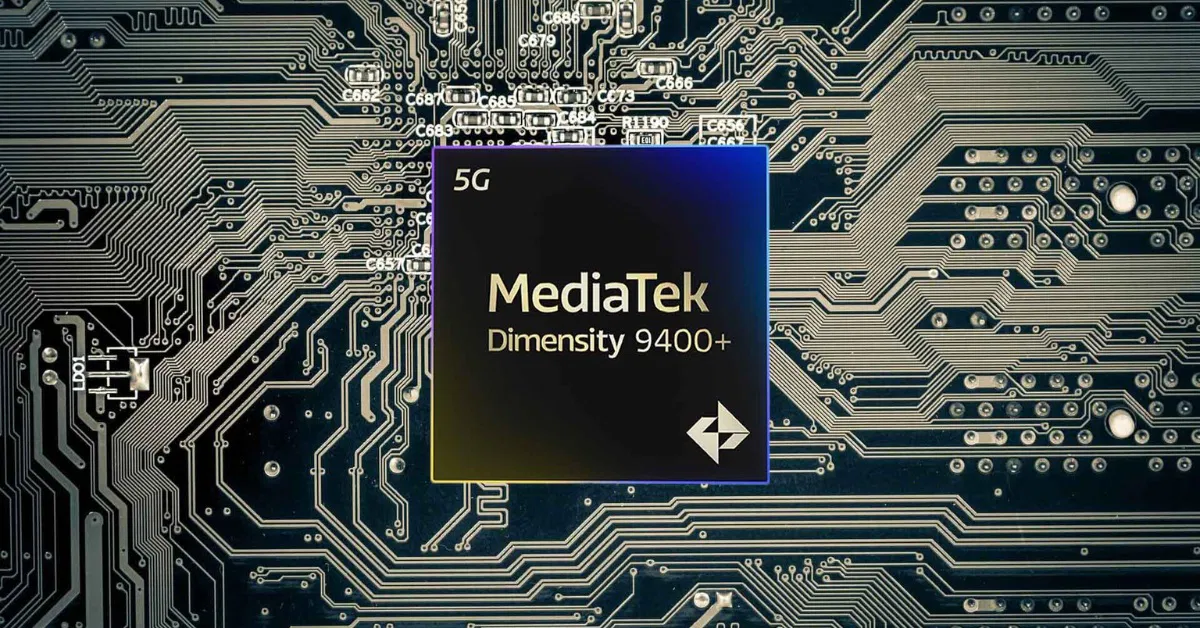
\includegraphics[width=0.9\linewidth]{img/cpu_mobile.png}
    \caption{Dimensity 9400 Plus của MediaTek đang là CPU Smartphone mạnh nhất hiện tại}
\end{figure}

\subsection{Bộ vi xử lý hệ thống nhúng (Embedded CPU/Microcontroller)}

\begin{itemize}
    \item \textbf{Đặc điểm chính}: Được thiết kế cho các nhiệm vụ chuyên biệt, độ tin cậy cao, chi phí thấp, tiêu thụ năng lượng cực thấp và thường hoạt động trong thời gian thực.
    
    \item \textbf{Kiến trúc phổ biến}: Rất đa dạng, bao gồm ARM (đặc biệt là dòng Cortex-M), MIPS, AVR, PIC và nhiều kiến trúc độc quyền khác. Lựa chọn kiến trúc phụ thuộc vào yêu cầu cụ thể của ứng dụng.
    
    \item \textbf{Vi điều khiển (Microcontroller - MCU)}: Trong nhiều hệ thống nhúng, "CPU" thực chất là một vi điều khiển. MCU là một vi mạch tích hợp bao gồm một lõi CPU, bộ nhớ chương trình (Flash/ROM), bộ nhớ dữ liệu (RAM), các bộ định thời (timers), bộ đếm (counters), các giao diện vào/ra (I/O ports), và các ngoại vi giao tiếp (UART, SPI, I2C).
    
    \item \textbf{Tài nguyên hạn chế}: Bộ nhớ (RAM, ROM) và tốc độ xử lý thường bị giới hạn để tối ưu chi phí và năng lượng.
    
    \item \textbf{Hệ điều hành thời gian thực (RTOS)}: Nhiều hệ thống nhúng, đặc biệt là những hệ thống yêu cầu đáp ứng tức thời và có tính quyết định (deterministic), sử dụng RTOS để quản lý tác vụ và đảm bảo thời gian phản hồi.
    
    \item \textbf{Firmware}: Phần mềm điều khiển cho hệ thống nhúng, được gọi là firmware, thường được lưu trữ trong bộ nhớ cố định (ROM hoặc Flash) và được thiết kế để thực hiện một tập hợp các chức năng cụ thể.
    
    \item \textbf{Tương tác với thế giới thực}: Thường được kết nối trực tiếp với các cảm biến (sensors) để thu thập dữ liệu từ môi trường và các cơ cấu chấp hành (actuators) để điều khiển thiết bị vật lý.
\end{itemize}

\begin{figure}[H]
    \centering
    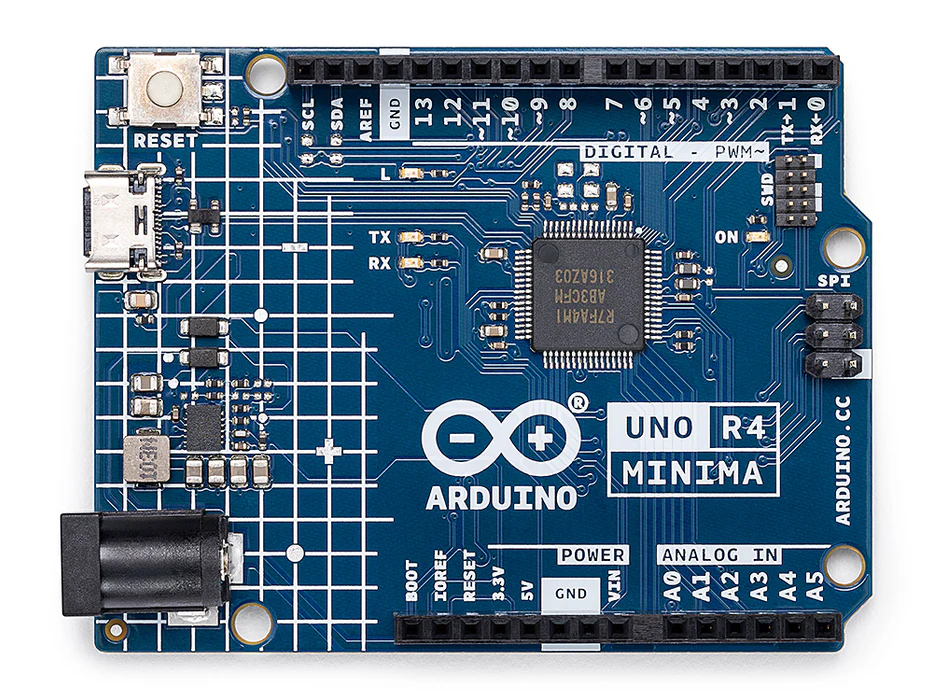
\includegraphics[width=0.65\linewidth]{img/cpu_embedded.png}
    \caption{Bo mạch Arduino}
\end{figure}

\subsection{So sánh CPU}

\begin{table}[H]
\centering
\label{tab:compare}
\begin{tabular}{|l|l|l|l|l|}
\hline
\textbf{Đặc điểm} &
  \textbf{PC CPU} &
  \textbf{Server CPU} &
  \textbf{Mobile CPU (SoC)} &
  \textbf{Embedded CPU/MCU} \\ \hline
\textbf{\begin{tabular}[c]{@{}l@{}}Mục tiêu \\ chính\end{tabular}} &
  \begin{tabular}[c]{@{}l@{}}Cân bằng \\ hiệu năng\\ /giá, đa năng\end{tabular} &
  \begin{tabular}[c]{@{}l@{}}Độ tin cậy, hiệu \\ năng song song, \\ sẵn sàng cao\end{tabular} &
  \begin{tabular}[c]{@{}l@{}}Tiết kiệm năng \\ lượng, tích hợp \\ cao, nhỏ gọn\end{tabular} &
  \begin{tabular}[c]{@{}l@{}}Chuyên biệt, chi phí \\ thấp, năng lượng thấp\end{tabular} \\ \hline
\textbf{\begin{tabular}[c]{@{}l@{}}Kiến \\ trúc\end{tabular}} &
  \begin{tabular}[c]{@{}l@{}}Chủ yếu x86 \\ (CISC)\end{tabular} &
  \begin{tabular}[c]{@{}l@{}}Chủ yếu x86 \\ (CISC), ARM \\ (RISC)\end{tabular} &
  \begin{tabular}[c]{@{}l@{}}Chủ yếu ARM \\ (RISC)\end{tabular} &
  \begin{tabular}[c]{@{}l@{}}ARM, MIPS, AVR, \\ PIC (đa dạng)\end{tabular} \\ \hline
\textbf{Số lõi} &
  \begin{tabular}[c]{@{}l@{}}Trung bình \\ (2-16+)\end{tabular} &
  \begin{tabular}[c]{@{}l@{}}Cao đến \\ rất cao\end{tabular} &
  \begin{tabular}[c]{@{}l@{}}Trung bình \\ (thường có kiến trúc \\ big.LITTLE)\end{tabular} &
  \begin{tabular}[c]{@{}l@{}}Thường là đơn lõi \\ hoặc ít lõi\end{tabular} \\ \hline
\textbf{Cache} &
  Khá lớn &
  \begin{tabular}[c]{@{}l@{}}Rất lớn, \\ nhiều cấp\end{tabular} &
  \begin{tabular}[c]{@{}l@{}}Vừa phải, tối ưu cho \\ năng lượng\end{tabular} &
  Nhỏ hoặc rất nhỏ \\ \hline
\textbf{\begin{tabular}[c]{@{}l@{}}Tích \\ hợp\end{tabular}} &
  \begin{tabular}[c]{@{}l@{}}iGPU, bộ điều \\ khiển bộ nhớ\end{tabular} &
  \begin{tabular}[c]{@{}l@{}}Bộ điều khiển \\ bộ nhớ, I/O \\ tốc độ cao\end{tabular} &
  \begin{tabular}[c]{@{}l@{}}CPU, GPU, ISP, \\ DSP, modem, \\ AI (NPU)...\end{tabular} &
  \begin{tabular}[c]{@{}l@{}}CPU, RAM, ROM, \\ I/O, ngoại vi trên \\ một chip\end{tabular} \\ \hline
\textbf{\begin{tabular}[c]{@{}l@{}}RAM \\ hỗ trợ\end{tabular}} &
  \begin{tabular}[c]{@{}l@{}}Non-ECC, DDR \\ SDRAM\end{tabular} &
  \begin{tabular}[c]{@{}l@{}}Thường là \\ ECC DDR \\ SDRAM\end{tabular} &
  \begin{tabular}[c]{@{}l@{}}LPDDR SDRAM \\ (Low Power)\end{tabular} &
  \begin{tabular}[c]{@{}l@{}}RAM nội bộ, có \\ thể có giao tiếp \\ RAM ngoài\end{tabular} \\ \hline
\textbf{\begin{tabular}[c]{@{}l@{}}Năng \\ lượng\end{tabular}} &
  \begin{tabular}[c]{@{}l@{}}Trung bình \\ đến cao\end{tabular} &
  Cao &
  Rất thấp đến thấp &
  Cực thấp \\ \hline
\textbf{Chi phí} &
  Trung bình &
  Cao &
  \begin{tabular}[c]{@{}l@{}}Trung bình \\ (tính trên SoC)\end{tabular} &
  Rất thấp đến thấp \\ \hline
\textbf{\begin{tabular}[c]{@{}l@{}}Xu \\ hướng\end{tabular}} &
  \begin{tabular}[c]{@{}l@{}}Tăng số lõi, \\ tích hợp AI, \\ kiến trúc chiplet\end{tabular} &
  \begin{tabular}[c]{@{}l@{}}Tăng số lõi, hiệu \\ quả năng lượng, \\ AI, chiplet\end{tabular} &
  \begin{tabular}[c]{@{}l@{}}Tăng hiệu năng AI, \\ 5G, hiệu quả \\ năng lượng\end{tabular} &
  \begin{tabular}[c]{@{}l@{}}Kết nối IoT, bảo mật, \\ AI tại biên (Edge AI)\end{tabular} \\ \hline
\end{tabular}
\caption{So sánh CPU trên các loại thiết bị khác nhau}
\end{table}